\documentclass[10pt,a4paper]{article}
% ========================== DO NOT MODIFY =================================== %
\usepackage[a4paper,left=2.0cm,top=2.0cm,right=2.0cm,bottom=2.0cm]{geometry} 
\usepackage{amssymb,amsmath} % If amsmath is required
\usepackage{url}
\usepackage{times}
\usepackage{mathptmx}      %% use fitting times fonts also in formulas
\usepackage{graphicx}
\usepackage{titling}
\usepackage{authblk}
\usepackage{multicol}
\usepackage{float}
\usepackage{enumitem}
\usepackage[small,compact]{titlesec}
\usepackage[numbers,sort&compress]{natbib}
\usepackage[T1]{fontenc}
\usepackage[UKenglish]{babel}
\usepackage[small,bf,tableposition=top,figureposition=bottom,skip=2pt]{caption}


% limit space between floats and text
\setlength{\textfloatsep}{10pt plus 1.0pt minus 2.0pt}
% shrink the list environments
\setlist{noitemsep}
\setlist{nolistsep}

% Shrink the bibliography
  \let\oldthebibliography=\thebibliography
  \let\endoldthebibliography=\endthebibliography
  \renewenvironment{thebibliography}[1]{%
    \begin{oldthebibliography}{#1}%
      \setlength{\parskip}{0ex}%
      \setlength{\itemsep}{0ex}%
  }%
  {%
    \end{oldthebibliography}%
  }

% Format of the front matter
\renewcommand{\Affilfont}{\small}
\setlength{\affilsep}{1ex}
\renewcommand\Authands{, }
\setlength{\droptitle}{-1.634cm}
% ============================================================================ %


% To be able to type european characters without escape sequences
% uncomment according to your operating system, if desired:
% ---------------------------------------------------------------------------- %
% \usepackage[latin1]{inputenc}   %% (Windows, old Linux)
% \usepackage[utf8]{inputenc}     %% (Linux)
% \usepackage[applemac]{inputenc} %% (Mac OS)
% ---------------------------------------------------------------------------- %


%------------------------------- FRONT MATTER -------------------------------- %
\title{%
Conductivity perturbations in EIT
\vspace{-2ex}} %remove vertical space
\author[1]{Andy Adler}
\author[2]{William R.B. Lionheart}
\affil[1]{Systems and Computer Engineering, Carleton University, Ottawa, Canada}
\affil[2]{School of Mathematics, University of Manchester, UK}
\date{}
%----------------------------------------------------------------------------- %



\begin{document}
\maketitle
\vspace{-1.5cm}
\thispagestyle{empty}

\begin{multicols}{2}

\noindent {\bf Abstract:}
Difference EIT reconstructs a signal generated
by conductivity contrasting regions. We explore
the effect that, for large contrasts, conductive regions
produce a greater signal than non-conductive ones,
and this difference is determined by the region shape.


\section{Introduction}
EIT images conductivity contrasting regions within a body.
Image reconstruction algorithms (especially for difference
imaging) are based on linearization of the sensitivity matrix.
For this reason, the sensitivity of EIT to small contrasts
is well understood. A small change of
 $\sigma + \Delta \sigma$
produces the same magnitude of signal change as
 $\sigma - \Delta \sigma$ 
(or, in logarithmic space,
 $\sigma^{1+\Delta}$ and 
 $\sigma^{1-\Delta}$).
However, in practice, conductivity contrasts can be large
(i.e.\ air in the lungs, or hypertonic saline in the blood).

In this paper we seek to understand the strength of EIT signals as a
function of the conductivity contrast ratio.
Our analysis is based on a simplification that
the target is far from measuring electrodes relative to its size
(which is reasonable for many biomedical applications of EIT). 
In this case, the contrast can be understood in terms of the
polarization tensor, for which there is a well developed theory\cite{amari2007}.


\section{Perturbations and current streamlines} 
Perhaps surprisingly, the most important factor is the shape
of the target area with respect to the current stream lines.
A non-conductive target has most effect when it is mostly 
perpendicular to the streamlines, while, for a conductive target,
the effect is largest when parallel.


In order to illustrate this effect,
we simluate an elliptical region of conductivity,
$\sigma$, in an otherwise homogeneous rectangular region of unity conductivity.
Two electrodes are placed at each horizontal end to produce 
a horizontal voltage gradient.
As shown in Fig.\ref{fig:streamlines}, for a non-conductive contrast
(top row, with $\sigma\approx.05$), the most significant effect is when the
major axis of the ellipse is oriented perpendicular to the streamlines. 
On the other hand, for a conductive contrast (bottom row, with $\sigma\approx20$), the
most significant effect is the converse, when the major axis is parallel
to the streamlines.


\begin{figure}[H]
\centering
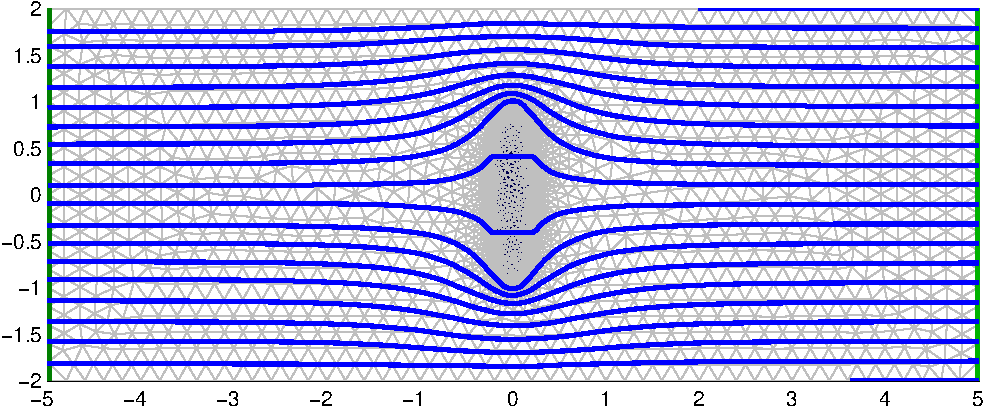
\includegraphics[width=.50\columnwidth,trim= 0 10 0 0,clip]{contrasts_04b.pdf}%
\hspace{0.5mm}
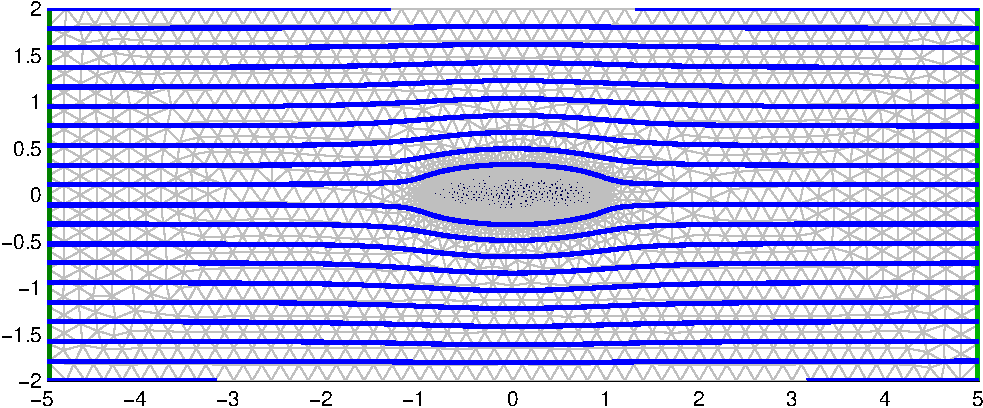
\includegraphics[width=.478\columnwidth,trim=19.5 10 0 0,clip]{contrasts_04p.pdf}%
\vspace{0.5mm}
\\
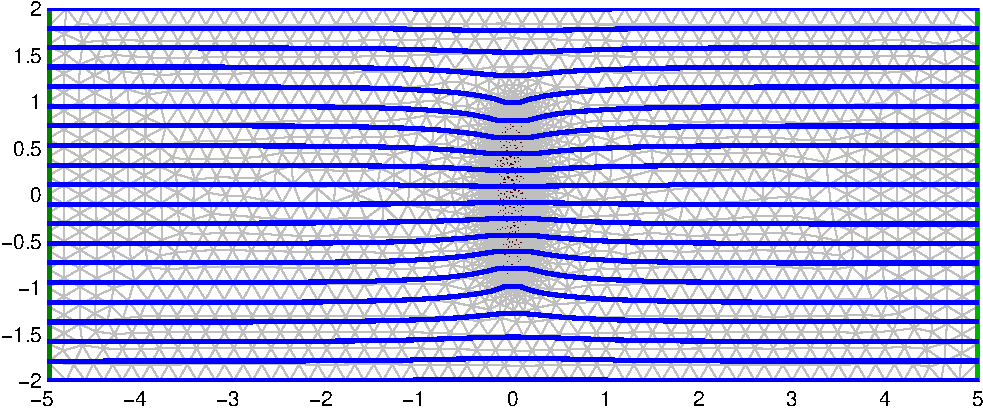
\includegraphics[width=.50\columnwidth,trim= 0  0 0 0,clip]{contrasts_04h.pdf}%
\hspace{0.5mm}
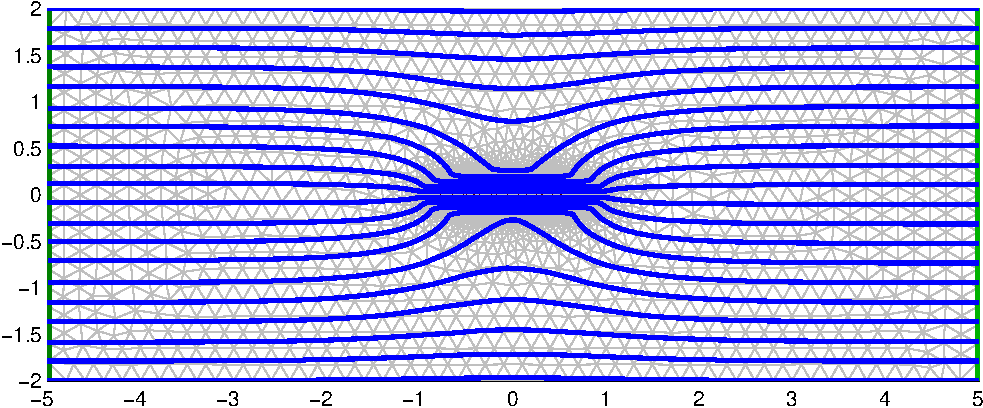
\includegraphics[width=.478\columnwidth,trim=19.5  0 0 0,clip]{contrasts_04v.pdf}%
\caption{\label{fig:streamlines}%
Streamlines surrounding an elliptical inclusion of various contrasts in 2D. 
The elliptical horizontal/vertical major axis dimension is 
{\em left column}: 2.0
and 
{\em right column}: 0.5.
The contrast/background ratio was 
{\em top row (non-conductive)}: exp($-3.0$)$\approx.05$ 
and 
{\em bottom row (conductive)}: exp($+3.0$)$\approx20$.
}
\end{figure}

  This makes intuitive sense. A contrasting region which which blocks
the streamlines will have the most effect when it is non-conductive.
However, a region which follows close to the streamlines will,
if conductive, draw in the streamlines, but, if non-conductive, have
little effect.

\section{Conductivity contrasts and EIT}

In order to understand the how this effect manifests itself into
an EIT system in 3D, we consider a simplified chest model as a cylinder
with 16 electrodes in a central plane (with hight/diameter ratio of one).
A small central ellipsoidal region is created as a conductivity contrasting
target. The ellipsoid has a circular cross section in the electrode
plane (with radius 0.1) but with a parameterized semi-axis length, 
$z= 0.1*r$ in the vertical direction. The cylinder had unity conductivity,
except for the ellipsoid, with conductivity $\sigma$.

A difference signal
 $s(z,\sigma)=\|{\bf v}(z,\sigma) - {\bf v}_h\|_2$
 was calculated, where ${\bf v}(z,\sigma)$ is the vector
of EIT measurements using adjacent simulation and measurement
for ellipsoid vertical dimension $z$ and conductivity $\sigma$,
and ${\bf v}_h = {\bf v}(z,1)$ is the corresponding homogeneous signal.

The signals normalized to their maximum values are shown in Fig\.~\ref{fig:graph}.
A similar effect is shown as before. A flat ellipse gives a much larger
signal for conductive contrasts, while, as the ellipse becomes tall, the
non-conductive contrast increases (with an equal effect when the ellipse
becomes a infinite vertical cylinder).


\begin{figure}[H]
\centering
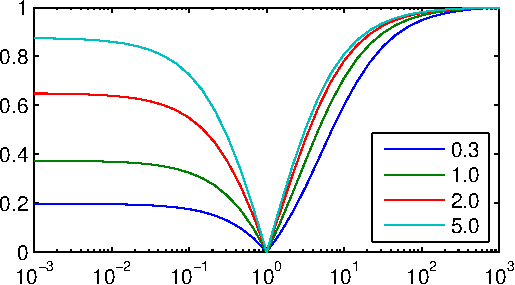
\includegraphics[width=.96\columnwidth]{signal.pdf}
\caption{\label{fig:graph}%
Normalized EIT signal, $s(z,\sigma)$ versus conductivity contrast, $\sigma$, for
different ellipsoidal vertical semi-axis ratios, $r$.
}
\end{figure}


\section{Discussion}

We show that the signal amplitude saturates differently for 
conductive and non-conductive targets, and this difference
depends on the object shape. A complete theory of this
effect has been developed by \cite{amari2007}, in which 
the polarization tensors for 2D ellipses (eqn 4.11) and 
ellipsoids (eqn 4.14) are given.

\footnotesize
\begin{thebibliography}{}
\bibitem{amari2007} 
Amari H, Kang H, 
Polarization and Moment Tensors: with Applications to
Inverse Problems and Effective Medium Theory. Applied Mathematical
Sciences Series, Vol 162, Springer-Verlag, 2007.
\end{thebibliography}
\end{multicols}



\end{document}
